
\documentclass[12pt,a4paper,titlepage]{report}
%\documentclass[a4paper,12pt]{article}
\usepackage[utf8x]{inputenc}
\usepackage{amsfonts}
\usepackage{fancyhdr}
\usepackage{titlesec}
\usepackage{tocloft}
\usepackage{listings}
\usepackage[T1]{fontenc}
\usepackage{ascii}
\usepackage{graphicx}
\usepackage{pifont}
\usepackage{float}
\usepackage{sidecap}
\usepackage{wrapfig}
\usepackage{titletoc}
\usepackage{tocloft}
\usepackage[nottoc]{tocbibind}
\usepackage{afterpage}
\usepackage[right=25mm,left=35mm,top=25mm,bottom=25mm]{geometry}
\usepackage[parfill]{parskip}
\usepackage{comment} 
%\usepackage[a4paper]{geometry}
\usepackage[numbers]{natbib}
\usepackage{balance}
\usepackage[table]{xcolor}
\usepackage{color}
\usepackage{amsmath}
\usepackage[inference,shorthand]{semantic}

\newcommand{\hilight}[1]{\colorbox{yellow}{#1}}	
\addtocontents{toc}{\protect\renewcommand{\protect\cftchapleader}{\bfseries\protect\cftdotfill{\protect\cftdotsep}}}
\newenvironment{cmd}{\fontfamily{ascii}\footnotesize\selectfont}{}
\setcounter{secnumdepth}{3}
\setcounter{tocdepth}{3}

\titleformat{\chapter}[hang]{\huge}{\thechapter}{1em}{}
\titlespacing{\chapter}{0pt}{0pt}{1cm}

\pagestyle{fancy}
\fancyhead{}
\fancyfoot{}

\setlength{\headheight}{15pt}
\addtolength{\textwidth}{2cm}
\addtolength{\hoffset}{-1cm}

\fancyfoot[C]{\thepage}
\renewcommand{\headrulewidth}{0pt} 
\renewcommand{\chaptername}{}


\begin{document}



%%%%%%%%%
%%%%%%%%%%%%%%%%%%%% Title page %%%%%%%%%%%%%
%%%%%%%%%

\begin{titlepage}
\vspace*{\fill} % Vertical Align
\begin{center}

% Uni stuff


%	LOGO SECTION
%----------------------------------------------------------------------------------------


\includegraphics[width=0.5\textwidth]{logo.jpg}\\[1.4cm] 

%----------------------------------------------------------------------------------------



% Title
\textbf{\LARGE Platform for Microrobot Navigation} \\ [1.5cm]


% Author and date
{\LARGE Nafiseh Vahabi} \\ [1.3cm]


% Report title
{\LARGE \lq{}\lq{}A thesis submitted in partial fulfilment of the } \\ [0.3cm]
{\LARGE requirements for the degree of MRes in }\\ [0.3cm]
{\LARGE  Medical Robotics and Image Guided Intervention}\\ [0.3cm]
{\LARGE  and for the Diploma of Imperial College\rq{}\rq{}}\\ [1.3cm]


{\LARGE Imperial College London} \\ [0.8cm]

{\LARGE \today} \\ [1.5cm]

% Examiner details
{\LARGE Project supervisors: Dr. Henry lp, Dr. Vincenzo Curto} \\ [0.3cm]
{\LARGE and  Professor Guang-Zhong Yang} \\ [1cm]




\end{center}
\vspace*{\fill}
\end{titlepage}

%%%%%%%%%
%%%%%%%%%%%%%%%%%%%%END Title page %%%%%%%%%%%%%
%%%%%%%%%

%\pagenumbering{roman}

%\section{Acknowledgements}
\addcontentsline{toc}{chapter}{\numberline{}Acknowledgements}
%\pagenumbering{roman}
%\setcounter{page}{1}
%\thispagestyle{plain}
\chapter*{Acknowledgements}
\pagebreak


\renewcommand{\cftsecleader}{\cftdotfill{\cftdotsep}}
\tableofcontents
%\setcounter{secnumdepth}{2}
%\setcounter{page}{1}

\pagebreak



\addcontentsline{toc}{chapter}{\numberline{}List of Figures}
%\setcounter{page}{3}
%\thispagestyle{plain}
%\listoffigures
\chapter*{List of Figures}
\pagebreak



\addcontentsline{toc}{chapter}{\numberline{}List of Tables}
%\setcounter{page}{2}
%\thispagestyle{plain}
%\listoftables
\chapter*{List of Tables}
\pagebreak

%------------------------------------------- Abstract -------------------------------------

\begin{abstract}
\addcontentsline{toc}{chapter}{\numberline{}Abstract}
%abstract

%\pagenumbering{roman}
%\setcounter{page}{2}
\thispagestyle{plain}

\end{abstract}

%-------------------------------------------END Abstract -------------------------------------




%%%%%%%%%
%%%%%%%%%%%%%%%%%%%% Introduction %%%%%%%%%%%%%
%%%%%%%%%
\chapter{Introduction}
Magnetically actuated helical micromachines can be used
 in a variety of biomedical applications such as cell characterisation, targeted drug delivery and in vivo 
diagnosis ~\citep{peyer2013magnetic}. However, the extremely small size of the microrobots and the
complex biofluid environment make the design aspect
very challenging. The two main difficulties are the power source and finding suitable locomotion methods, as
 there are many cells, proteins and fibres in biofluids that prevent the motion of the microrobots. 
The common method of using an external magnetic field produced the most successful result \hilight{[EVIDENCE]} ~\citep{peyer2013bio}. 

\paragraph{}
The design of microrobots depends on their application and the desired task. An overview of the different
 microrobot designs, their structures and fabrication methods are discussed in the chapter 2, literature review, .

\paragraph{}
For the purpose of this project different proposed structures of microrobots were studied
 and analysed. This will enable helical microswimmers to be reproduced. Once reproduced, the aim of this project will be to compare
 the efficiency, power, motion velocity and cost-efficiency of various microrobot designs for mass production
 of the microswimmers. The fabrication of microswimmers will be by Nanoscribe facility using 3D laser
 lithography. After the microrobots are produced their characteristic will be analysed
 under the scanning electron microscope in order to identify further improvements in microrobot design. 

\section{Problem}

\section{Previous work}


%%%%%%%%%
%%%%%%%%%%%%%%%%%%%% literature review %%%%%%%%%%%%%
%%%%%%%%%

\chapter{Literature review}
 


\section{Bioinspired microrobots}

One of the most challenging aspects of designing a robot on a very small scale such 
as a nanorobot is simplicity. The reason is, integration will become unfeasible on that
 scale if the design is complex. Hence the development of the nanorobot or even microrobot
 should be based on the essential functionality, avoiding any unnecessary components~\citep{gao2013bioinspired}.
By learning from nature and mimicking the structure of live organisms, the successful  
scientific applications were created~\citep{qiunanohelices}. In the following section a
 few examples of microrobots that were imitated from nature will describe. 
 



\paragraph{Reynolds number}

To understand how micro organisms swim in a fluidic environment, it is essential to study their propulsion 
mechanism. In the fluidic regime the Reynold number (Re) has a substantial effect on a microdevice
locomotion~\citep{peyer2013magnetic}. The Reynolds number describes the ratio of the inertial forces versus viscous 
forces according the following formula;

\begin{equation}
  Re = \cfrac{UL\rho}{\mu}
\label{eq:4}
\end{equation}
 
Where $ U$ is velocity, $L$ is characteristic length, $\rho$ is the density and $\mu$ is viscosity of the fluid.






\subsection{Flagella style microrobots}

Helical flagella and cilia are two well-known microswimers in nature that have had their functionality employed 
for motion generation in artificial microrobots  (Figure~\ref{cilia}) ~\citep{gao2013bioinspired}. 



\begin{figure}
  \centering
    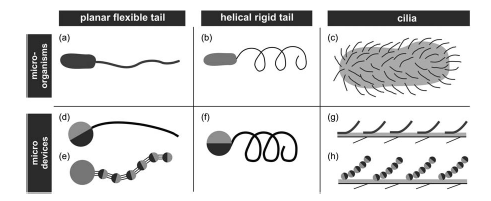
\includegraphics[width=0.9\textwidth]{cilia}
  \caption{The illustration of both flagellum and cilia shapes and microdevices mimicked the flagellum and cilia 
structures.~\citep{peyer2013bio}.}
  \label{cilia}
\end{figure}

In 2007, Bell ~\citep{gao2013bioinspired} presented the first artificial bacteria flagellum microrobots and then
 Zhang characterised them in 2009 ~\citep{gao2013bioinspired}. This microrobot was formed of two 
components; a rigid helical tail and a soft magnetic metal head. The head diameter 
was $2.8 \mu  m$ and its length was $30-100 \mu m$. Since then, other scientists proposed a slightly different design 
structure, that all have the rigid helical tail structure. However, in some cases the magnetic
 materials is used in the device tail rather than the head ~\citep{gao2013bioinspired}. 
 
\paragraph{}

%\begin{figure}
%  \centering
\begin{wrapfigure}{r}{0.5\textwidth}
  \begin{center}
    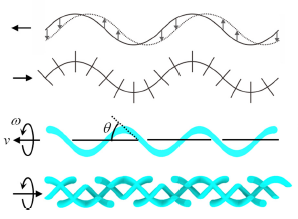
\includegraphics[width=0.5\textwidth]{10}
  \caption{ The structure of the smooth flagellum and a mastigonemes flagellum.~\citep{gao2013bioinspired}.}
  \label{10}
\end{center}
\end{wrapfigure}
%\end{figure}

The helical rotation of flagella and the travelling wave beat of cilia are two non-reciprocal propulsion
 mechanisms in microorganisms. Mimicking a rotating flagellum at low Reynolds number to generate an 
adequate torque to overpower the high viscous drag requires two main elements; a rotary motor and a
 power source ~\citep{qiunanohelices}. 
An electromagnetic rotary motor can be used in designing a helical flagella style microrobot that 
requires a considerable current. However piezoelectric rotary motors are an alternative option 
that are appropriate for miniaturisation but necessitate high input voltage.  Hence, designing a microrobot with a 
combination of an onboard power source and a motor is a challenging task ~\citep{qiunanohelices}.

Another design of microswimmers was inspired by the function of magtigonemes in nature ~\citep{tottori2013artificial}.
 A smooth flagellum moves against the direction of the propagation of the flagella wave. However, 
the flagellum covered by magtigoneme propels in the same direction as the flagellum wave (Figure~\ref{10}). Mimicking 
the structure of flagellum and using 3D lithography and electron beam evaporation formed the fabrication 
method in these microswimmers.
The anisotropic viscous drag on the flagella is an important fact for locomotion in low Reynolds number fluid. 
Flagella movement in the opposite direction of the flagella wave is because the 
viscous drag coefficient perpendicular to the flagella is greater than the viscous drag coefficient parallel to 
the flagella~\citep{tottori2013artificial}. 

 The rotating field, i.e. rotational frequency, field strength and angles that 
defined the rotational axis can be controlled by the current in the external coil. The helical microrobots rotate 
synchronously with the rotation of the magnetic field and move forward and backward accordingly ~\citep{tottori2013artificial}. 
The displacement of the microswimmer along the rotational axis can be measured and the result 
used to calculate the average velocity of the swimmers. There is a linear relationship between an input 
field frequency and swimming speed. According to their result ~\citep{tottori2013artificial}, a propulsive force generated by 
the mastigoneme is in opposite direction of the force generated by the main helical filament. 
However, this velocity is only valid if the external force is zero. The proposed 
design ~\citep{tottori2013artificial} is rigid and an external stimulus may be used to regulate the swimming
 speed and direction if the swimmer can fold and unfold their structure. 


There are three common shapes of microrobots 
based on the rotary action; a helix, a screw and a twisted ribbon shape around its
 axis (Figure~\ref{HelixShapes}). For the purpose of drilling into solid matter such as biological tissue the screw and helix 
design would be more appropriate. The rotational motion of helical micro
 swimmers is one of the most effective propulsion methods in the low Reynolds number scenarios 
because it leads to translational motion. Microrobots with the microspheres structure perform similarly 
to the helical swimmers and are capable of swimming in the flowing liquid within the microfluidic channel~\citep{kim2013fabrication}. 


%\begin{figure}
%\begin{SCfigure}
  %\centering
\begin{wrapfigure}{r}{0.5\textwidth}
  \begin{center}
    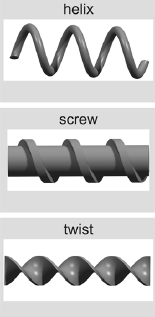
\includegraphics[width=0.4\textwidth]{HelixShapes}
  \caption{Three design of helical microswimmers.~\citep{peyer2013magnetic}.}
  \label{HelixShapes}
  \end{center}
\end{wrapfigure}
%\end{SCfigure}
%\end{figure}



There are two main factors that affect the movements of the microrobot in the external magnetic
 field; \hilight{low coercivity and high saturation} magnetization. Also, the motion of the microrobot is related to 
its size given the same magnetic field strength and as such, by increasing the size of the microrobot with the inflexible magnetic material
 volume, the velocity will decrease ~\citep{kim2013fabrication}. 
The surface friction and the drag forces are two resistive forces that impede the microrobot\rq{}s 
motion. Hence, the input magnetic force must be sufficient to overcome these forces for microrobot 
manipulation. Furthermore, the weight of the microrobot requires gravity compensation in the z-direction by 
the magnetic field. The navigation methodology should compensate for gravity to avoid sinking and enable velocity to be 
controlled wirelessly. \citeauthor{mahoney2011velocity} described an algorithm for helical microswimmers velocity 
control plus gravity compensation. In the proposed model the correct pitch angel and 
rotation speed is calculated to achieve the commanded velocity (Figure~\ref{11}).


\begin{figure}
  \centering
    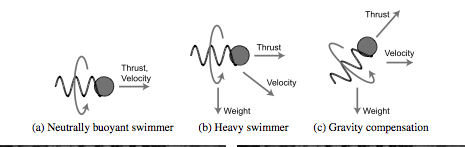
\includegraphics[width=0.9\textwidth]{11}
  \caption{The effect of the gravity on the microrobot motion direction and gravity compensation~\citep{mahoney2011velocity}.}
  \label{11}
\end{figure}


The mathematic model below describes the microrobot translational movement;

\begin{equation}
  \overrightarrow{F_m }+ \overrightarrow{F_r} - \overrightarrow{F_g} = M(\overrightarrow{dv}/dt)
\label{eq:4}
\end{equation}

Where $F_m$, $F_r$ and $F_g$ are a magnetic force, overall resistive force and gravitational force respectively. 
$M$ is a mass and $v$ is a translational velocity of the microrobot~\citep{kim2013fabrication}. 

A magnetic field can be used for controlling teams of microrobots as well as a single 
one. \citeauthor{kim2013fabrication} proposed a method that used a combination of two magnetic materials to 
attain on/off magnetization of each microrobot. The overall control of the group of microrobots 
was achieved by managing the magnetization state of each microrobot. In addition, a second technique has been 
developed for three-dimensional motion of the team of microrobots in a fluidic environment. In
 the latter method, each microrobot is designed in such a way that it uniquely responds to the 
input magnetic field. Therefore, several microrobots can provide feedback position control in 
3D system~\citep{kim2013fabrication}.
An untethered spherical magnetic micromanipulator creates a locally induced rotational fluid flow gradient. 
The created rotational flow propels micro-objects in the flow area. A team of microrobots could perform
 a complex task in micro-transport and micro-assembly~\citep{kim2013fabrication}.

In another study ~\citep{tottori2012magnetic}, a helical microrobot was designed to swim in a low Reynolds number. 
Two designs are selected to run the experiment;  the first one is a bare helical structure and the second one is the
 helical shape with the microholder attached at the end. Both designs will generate the corkscrew
 motion in a fluid environment when the magnetic filed is about few mili Tesla. The second 
design (device with the microholder) is capable of transporting a microobject accurately to the 
target ~\citep{tottori2012magnetic}.\hilight{size and weight of the object}


%\begin{figure}
  %\centering
\begin{wrapfigure}{r}{0.5\textwidth}
  \begin{center}
    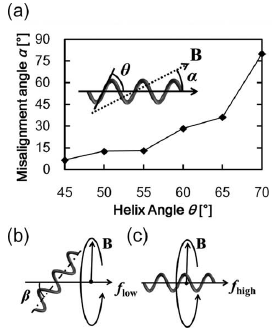
\includegraphics[width=0.5\textwidth]{7}
  \caption{(a) The misalignment of helical angle$\alpha$ with differnt helix angle (b) the oscillation behaviour
of the microswimmer with the high and low frequencies ~\citep{tottori2012magnetic}.}
  \label{ref7}
\end{center}
\end{wrapfigure}
%\end{figure}


In ~\citeauthor{tottori2012magnetic}\rq{}s study eight designs of microrobots were proposed and tested. 
The uniform static magnetic field was used to explore the magnetic shape anisotropy and the 
magnetic actuation was monitored in the rotating magnetic field. In the static magnetic field the 
set of microrobots had helical angles $\theta$ ranging from ${45^{\circ}}$ to ${70^{\circ}}$ when suspended in the deionised water. 

This showed (Figure~\ref{ref7}) that a smaller helix angle $\theta$ results in a less misalignment 
angle $\alpha$ because microrobots longest axes will be aligned to the direction of the external magnetic field. 
However in helical microrobot with larger helix angles ($\theta$), the magnetization direction would change to 
the radial axes of the helix  ~\citep{tottori2012magnetic}.
In the rotating magnetic field, the micro helical swimmer exhibits different behaviours depending on 
the strength of the applied frequency in the fixed magnetic field. At low frequencies the micro helix oscillated 
around the helical axes, however the oscillating behaviour changed to the 
corkscrew motion after increasing the applied frequency in the magnetic field. This is similar to characteristics of 
microrobots with an incorporated
 microholder~\citep{tottori2012magnetic}.

The velocity of helical micro swimmers depends on their size and shape. A linear relationship was 
observed between the input frequencies and swimming velocity of the micro swimmers. The outcome of 
the comparison between three microhelixs with the same helix angles showed that the microhelix with the
 greatest diameter has the highest speed, in accordance with the following formula;

\begin{equation}
  U = {\cfrac{(C_n - C_1) \sin \theta \cos \theta}{2(C_n \sin^2 \theta + C_1 \cos^2 \theta)}} \big( d \varpi \big)
\end{equation} 

Where $C_n$ is a drag coefficient perpendicular to the filament and $C_1$ is a drag coefficient
 parallel to the filament. $ \varpi$ is the rotational frequency and $d$ is the rotational diameter of 
the helix ~\citep{tottori2012magnetic}.  



\paragraph{}
The important role of helix angle in the magnetization structure of helical micro swimmers 
was confirmed by \citeauthor{peyer2013bacteria}, who used direct laser writing (DLW) as a fabrication method but 
applied (DLW) on a magnetic polymer composite (MPC). The MPC are non-cytotoxic and showed 
super paramagnetic characteristic because magnetic material was already included in the polymer. 

The relationship between the torque $T_d$, the drag force $F_d$, the object\rq{}s velocity $U$ and rotational 
speed $\omega$ is linear and modelled by $6\times6$ resistant matrix as below;



\[
\begin{bmatrix} F_d \\ 
T_d \end{bmatrix}  =- \begin{bmatrix} A & B \\ 
B^T & C \end{bmatrix}  \begin{bmatrix} U
 \\ \omega
\end{bmatrix}
\]




Where $A$, $B$ and $C$ are matrices 3x3 and only depend on the object\rq{}s geometry and fluid velocity. 
There are few methods in use to model the resistance matrices and low Reynolds flow such as the 
method of regularized stokeslets, the boundary element method and the method of fundamental solution
. In designing a microrobot the main parameters required to concentrate on are the helicity angle $\psi$, 
the helix radius $R$, the pitch $p$ and the filament radius $r$ as illustrated in Figure~\ref{ref8} part (c). 
The details of above methods will discuss in section 3.2.1 (Mathematical model).

\begin{figure}
  \centering
    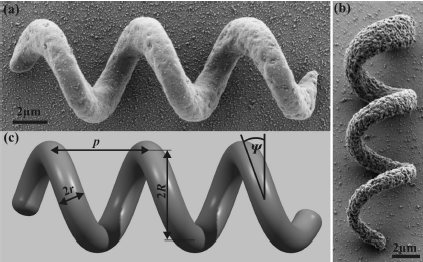
\includegraphics[width=0.7\textwidth]{8}
  \caption{ The prototype of microhelical device. (a) Scanning electron microscopic image of the micro polymer composite
with the 2 vol.\% nanoparticle fill factor and (b) 4 vol.\% of nanoparticle fill factor. (c) The CAD model
shows all the parameters required for the microhelical design ~\citep{peyer2013bacteria}.}
  \label{ref8}
\end{figure}

Magnetic actuated microrobot is divided into two categories; torque driven microrobot and force
 driven microrobots.
The micro robot using the torque-driven method is more favourable than the force-driven method 
because their rotation is based on applying torque rather than a force to pull the device ~\citep{peyer2013bacteria}.

Another approach for powering a micro robot is using the catalytic conversion of chemical energy
 into mechanical energy (Figure~\ref{nanotube}). In this method, the catalyst accelerates the consumption of hydrogen peroxide
 and helps the self-propulsion of micro robot to pump the fluid to transport cells and colloidal 
particles ~\citep{C2NR32798H}.

The catalytic tube is fabricated with a sub micrometer diameter.
 This technique is not applicable for the minimally invasive surgery (MIS) yet because the catalytic
 material used in the fabrication process of nanotubes is toxic. Hence, biocompatible fuel is required to be developed in order to 
apply this technique in a live cell environment~\citep{C2NR32798H}.


%\begin{figure}
%  \centering
\begin{wrapfigure}{r}{0.5\textwidth}
  \begin{center}
    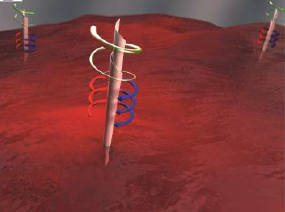
\includegraphics[width=0.5\textwidth]{nanoJet3}
  \caption{Demonstrating the drilling motion of the nanotubes under rotating
 magnetic field~\citep{C2NR32798H}.}
  \label{nanotube}
\end{center}
\end{wrapfigure}
%\end{figure}

Alternatively, the micro driller can be powered and controlled by using an external magnetic field 
such that changes in the frequency of the rotating magnetic field switch the rotational orientation of the 
micro tool from the horizontal position to the vertical one. The vertical orientation of the rolled up microtube 
and its sharp helical design makes the device suitable for drilling into biological tissue. In addition, the micro 
driller can be used for targeted drug delivery in MIS ~\citep{C2NR32798H}. 


\subsection{Plant-based microrobots}
\hilight{details about fabrication, extract xylem tissue}
The helical microstructures are not limited to having flagellum-like structures and microbots with
general cilia-like feature have been designed. \citeauthor{gao2013bioinspired}
 observed the helical microstructures that imitates spiral water-conducting vessels of different plants. 

\begin{figure}
  \centering
    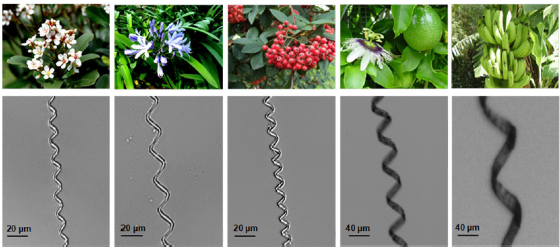
\includegraphics[width=0.9\textwidth]{plants}
  \caption{The shape of the Xylem in differnt plants .~\citep{mahoney2011velocity}.}
  \label{plants}
\end{figure}



The fabrication process involves coating isolated spiral xylem vessel plant fibres within a (Figure~\ref{ref8})
thin magnetic layer. Xylem tissue transports the plant\rq{}s required food such as water and other 
nutrition from the root to the leaves using capillary action ~\citep{mahoney2011velocity}.
Use of plant material in this method enables simple three-dimensional microswimmers fabrication 
and biocompatibility. In addition, the magnetic cover helps to ensure accurate directional control and 
high-speed propulsion. Therefore the fabrication processes were extremely simplified as the main 
component of the helical microswimmers is from nature and more than a million individual micro helicals 
can be made from a very small section of the plant stalk ~\citep{mahoney2011velocity}. 


Using mechanical stretching can control geometric variables of the helical vessels such as the pitch and
 helix angle and hence plenty of helical microswimmers can be reproduced. The final shape of the 
helical microswimmer is determined mainly by the initial diameter of the unstretched spiral vessel. The
 process of stretching helical plant structure was performed via plastic deformation so that the number 
of helical turns are constant and tensile stretching of the plant fibre stretching is negligible~\citep{mahoney2011velocity}. 


%\begin{figure}
%  \centering
\begin{wrapfigure}{r}{0.5\textwidth}
  \begin{center}
    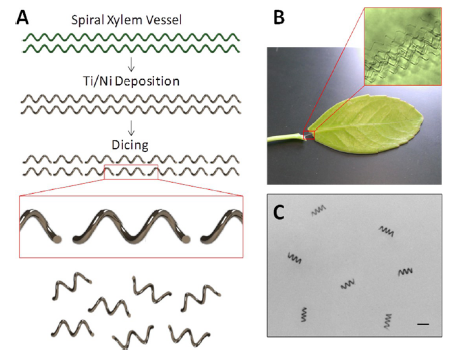
\includegraphics[width=0.5\textwidth]{plants2}
  \caption{(A) The stages were required to make a plant-based microrobot. (B) A microscopic image of the 
a xylem helical structure. ~\citep{gao2013bioinspired}.}
  \label{plants2}
\end{center}
\end{wrapfigure}
%\end{figure}


The method used for precise propulsion control and characterising the locomotion behaviour of the 
plant-based microswimmers is similar to the method applied in \citeauthor{gao2013bioinspired} study.

According to \citeauthor{gao2013bioinspired} experiment, the plant-based 
microswimmers exhibited high speed movement in raw biological medium such as 
pure human serum under the rotating magnetic field. Moreover, the increased velocity of the 
biological fluid has a minor effect on the plant-driven microswimmers, which is an important 
advantage of this microdevice over the common microrobots\hilight{WHY}.

\subsection{Jellyfish style microrobots}
For the purpose of this project different proposed structures of microrobots were studied
 and analysed. This will enable helical microswimmers to be reproduced. Once reproduced, the aim of this project will be to compare
 the efficiency, power, motion velocity and cost-efficiency of various microrobot designs for mass production
 of the microswimmers. The fabrication of microswimmers will be by Nanoscribe facility using 3D laser
 lithography. After the microrobots are produced their characteristic will be analysed
 under the scanning electron microscope in order to identify further improvements in microrobot design. 



\section{Fabrication methods}

Historically, the fabrication of the microrobot was the main problem that recent fabrication methods 
offer a feasible solution~\citep{gao2013bioinspired}. 
A typical fabrication process consists of two stages. Initially the core structure of the artificial helical 
microswimmer is printed using 3D lithography and then electron beam evaporation is used for 
ferromagnetic thin film coating~\citep{tottori2013artificial}.  
Performance of each microswimmer (with different design) can be imaged by the scanning electron
 microscope (SEM). After the fabrication process is completed, the next step is to release the structure into 
deionised water using the tungsten probe. The tank with deionised water is installed in the middle of the 
three-axis Helmholtz setup. 

To improve biocompatibility for in-vivo applications, the 
microrobot can be covered with a thin layer of titanium. In addition, the microrobot\rq{}s structure was layered with 
nickel for the purpose of magnetic actuation.


%%%%%%%%%%%%%%% Table %%%%%%%%%%%%%%
\begin{table}[h!]
  \centering

\setlength{\arrayrulewidth}{.6mm}
\setlength{\tabcolsep}{5pt}
\renewcommand{\arraystretch}{.8}


  \begin{tabular}{ c  m{3cm}  m{4.3cm} m{3cm} }
    \hline
\rowcolor{lightgray}
    Microrobot Image & Type  & Fabrication Method & Citation \\ \hline\hline
    \begin{minipage}{.3\textwidth}
      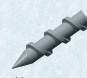
\includegraphics[width=\linewidth, height=25mm]{screw_ta}
    \end{minipage}
    &
    %\begin{minipage}[t]{5cm}
      \begin{itemize}
        \item Helical Screw Shape
    
      \end{itemize}
    %\end{minipage}
    & 
    %\begin{minipage}{5cm}
      \begin{itemize}
        \item Direct Laser Writting (DLW)
	\item Two-photon Polymerization
   
      \end{itemize}
    %\end{minipage}
	&
	   \begin{itemize}
        \item \citep{peyer2013magnetic}
   
      \end{itemize}
    \\ \hline
%%%%%%%%%% Second Row

 \begin{minipage}{.3\textwidth}
      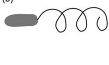
\includegraphics[width=\linewidth, height=25mm]{flagella_ta}
    \end{minipage}
    &
    %\begin{minipage}[t]{5cm}
      \begin{itemize}
        \item Flagella Shape
      
      \end{itemize}
    %\end{minipage}
    & 
    %\begin{minipage}{5cm}
      \begin{itemize}
        \item Direct Laser Writting (DLW)
	\item Two-photon Polymerization
   
      \end{itemize}
    %\end{minipage}
&
	   \begin{itemize}
        \item \citep{peyer2013bio}
   
      \end{itemize}
    \\ \hline

%%%%%%%%% Third Row
 \begin{minipage}{.3\textwidth}
      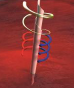
\includegraphics[width=\linewidth, height=25mm]{tube_ta}
    \end{minipage}
    &
    %\begin{minipage}[t]{5cm}
      \begin{itemize}
        \item Nanotube
        
      \end{itemize}
    %\end{minipage}
    & 
    %\begin{minipage}{5cm}
      \begin{itemize}
        \item Molecular Beam Epitaxy (MBE)
	   
	   
    
      \end{itemize}
    %\end{minipage}
	&
	   \begin{itemize}
        \item \citep{C2NR32798H}
   
      \end{itemize}
    \\ \hline

%%%%% Forth Row

 \begin{minipage}{.3\textwidth}
      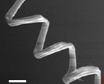
\includegraphics[width=\linewidth, height=25mm]{plant_ta}
    \end{minipage}
    &
    %\begin{minipage}[t]{5cm}
      \begin{itemize}
        \item Plant-based
      
      \end{itemize}
    %\end{minipage}
    & 
    %\begin{minipage}{5cm}
      \begin{itemize}
        \item Macerating Plant\rq{}s Leaves
	\item Seperating Spiral Vessels
	\item Stretching spiral Vessels
	\item Coating with Titanium

      \end{itemize}
    %\end{minipage}
	&
	   \begin{itemize}
        \item \citep{gao2013bioinspired}
   
      \end{itemize}
    \\ \hline

%%%%%% Fifth Row

 \begin{minipage}{.3\textwidth}
      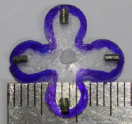
\includegraphics[width=\linewidth, height=25mm]{Jelly}
    \end{minipage}
    &
    %\begin{minipage}[t]{5cm}
      \begin{itemize}
        \item Jellyfish
     
      \end{itemize}
    %\end{minipage}
    & 
    %\begin{minipage}{5cm}
      \begin{itemize}
        \item The EMA coil system
     
      \end{itemize}
    %\end{minipage}
&
	   \begin{itemize}
        \item \citep{ko2012jellyfish}
   
      \end{itemize}
    \\ \hline



  \end{tabular}
  \caption{Different types of microrobots and their fabrication method.}\label{Micro}
\end{table}


%%%%%%%%%
%%%%%%%%%%%%%%%%%%%% Method %%%%%%%%%%%%%
%%%%%%%%%

\chapter{Methods}

%%%%%%%%%%%%%%%%%% Structure %%%%%%%%%%%%%
\section{Microrobot structure}


%%%%%%%%%%%%%%%%%%% Design %%%%%%%%%%%%%%%
\section{Microrobot design}
A rigid rotating helix is uesed as a reference to model a helical microrobot. The 
essential parameters to model a helix are, helix length ($L$), pitch ($\lambda$), pitch angle ($a$), 






\subsection{Mathematical model}
\subsubsection{Resistive force theory}
\subsubsection{Slender body theory}
\subsubsection{Regularized Stokeslet method}

%%%%%%%%%%%%%%%%%% Fabrication %%%%%%%%%%%%%
\section{Microrobot fabrication}
\subsection{}







%%%%%%%%%
%%%%%%%%%%%%%%%%%%%% Testing %%%%%%%%%%%%%
%%%%%%%%%
\chapter{Simulation, testing and validation}



%%%%%%%%%
%%%%%%%%%%%%%%%%%%%% Results %%%%%%%%%%%%%
%%%%%%%%%
\chapter{Results}



%%%%%%%%%
%%%%%%%%%%%%%%%%%%%% Discussion %%%%%%%%%%%%%
%%%%%%%%%
\chapter{Discussion}




%%%%%%%%%
%%%%%%%%%%%%%%%%%%%% Conclusion %%%%%%%%%%%%%
%%%%%%%%%
\chapter{Conclusion and future work}






\renewcommand{\bibname}{References}
\bibliographystyle{plainnat}
\bibliography{References} 
%\addcontentsline{toc}{chapter}{\numberline{}References}

\end{document}